%\documentclass[prd, nofootinbib, floatfix, 12pt]{revtex4}
%\documentclass[useAMS,usenatbib,11pt,preprint]{aastex}
\documentclass[]{article}

\usepackage[paperwidth=8.5in,paperheight=11in,centering,hmargin=1in,vmargin=1in]{geometry}
\usepackage{amsmath}
\usepackage{amsbsy}

\topmargin0.0cm
\textheight8.5in

\input epsf
\usepackage{amsmath,amssymb,subfigure}
\usepackage{graphicx}
\usepackage{epsfig}
\usepackage{color}
%\usepackage{ulem}
%\usepackage{epstopdf}

\renewcommand{\topfraction}{0.95}
\renewcommand{\bottomfraction}{0.95}





%%%%%%%%%%%%%%%%%%%%%%%%%%%%%%%%%%%%%%%%%%%%%%%%%%%%%%%%%%%%
%%%%%%%%%%%%%%%%%%%%%%%%%%%%%%%%%%%%%%%%%%%%%%%%%%%%%%%%%%%%
%%%%%%%%%%%%%%%%%%%%%%%%%%%%%%%%%%%%%%%%%%%%%%%%%%%%%%%%%%%%

\begin{document} 
\sloppy
\title
{Validation of the Simulations Catalogs}

%\pagerange{\pageref{firstpage}--\pageref{lastpage}}

\label{firstpage}

% \date{\today}

\maketitle 
\section{Introduction \label{sec:intro}}
The purpose of this document is to work in concert with the "Requirements for the 
LSST Simulation Framework" (hereafter Requirements; \cite{requirements}) to validate the
base catalogs and catalogs generation framework for use in the context of
LSST investigations. 

The simulations catalogs in combination with tools for applying astrometric effects and a 
framework for generating observed catalogs provide all the requisite tools for conducting a 
wide range of analysis activities.
\begin{itemize}
\item Realized positions of solar system objects can be used to test moving object detection algorithms.
\item Source catalogs can be used to test database and algorithm scaling.
\item Inputs generated for phosim using OpSim observing parameters allow for large scale image simulation
for sensitivity analysis and algorithm development.
\item Realistic base catalogs allow science collaborations to inject specialized objects for specific science
analysis.
\item Time domain catalogs of variable objects allow testing of lightcurve recovery and characterization.
\end{itemize}

All of the examples above require a set of base catalogs that are as realistic as possible.  The intention
is that the catalogs are representative in spatial distribution, color distribution, apparent
brightness distribution, and redshift distribution.  However, not all of these distributions have testable impacts
on the resulting science and operations.
The Requirements specify the aspects of the base catalogs that impinge measurably on science and 
operational drivers defined in the Science Requirements Document.

\section{Validation of the Requirements on the Catalog Simulations}
This section will show in detail whether each requirement is being met and if it is not
being met what the impact on the project measureables and design goals is.


\subsection{Requirement 1: The LSST catalogs simulations shall contain representations of stars,
galaxies, asteroids, and variable sources}
\subsubsection{Motivation}
The catalogs must provide representations of all object types important for testing the LSST system.  The base catalogs must
have:
\begin{itemize}
\item point sources -- PSF estimation and star galaxy separation
\item extended sources -- shape estimation and star galaxy separation
\item variabile sources -- alert production and lightcurve characterization
\item moving sources -- alert production and moving object detection
\end{itemize}

The base catalogs attempt to be as realistic as possible in implementing the distributions of these four types of objects.
Published models are used to populate the simulated sky.

\subsubsection{Stars}
Stars are represented as point sources.  SEDs and kinematics are assigned to stars using SDSS colors produced by the Galfast (\cite{galfast})
model.  Galfast generates stars according to the density laws in \cite{juric} which are derived from fitting SDSS data to a thick and thin disk along with a halo. Using this input and an input luminosity function Galfast samples stars from these distributions in a 4-dimensional probability density function $\rho$(x,y,z,M). After this stage, using Fe/H and kinematics models from \cite{ivezic} and \cite{bond} that are also derived from SDSS data, the stars are assigned further statistics along
with photometry in the desired bands. Finally, observational errors are added to account for the real-life properties of the telescope and the catalog is outputted. SEDs are matched to a star by a best-fit comparison in SDSS colors and come from 3 sources: 1) stars down to M-type dwarfs are from the Kurucz models, 2) M-type dwarfs come from \cite{bochanski} and 3) white dwarf spectra are from \cite{bergeron}. A three dimensional dust model is applied to un-extincted magnitudes using the smooth
model of \cite{amores} and normalizing to the
measured extinction values from \cite{sfd}.  Binary stars are included in the luminosity functions from which the stellar colors are sampled but are assumed to be unresolved and non-variable (except for a selection of eclipsing binarys described later).
%Stars are represented as point sources.  SEDs and kenimatics are assigned to stars using SDSS colors produced by the Galfast (\cite{galfast})
%model.  A three dimensional dust model is applied to un-extincted magnitudes using the smooth model of \cite{amores} and normalizing to the
%measured extinction values from \cite{sfd}.  Binary stars are included in the luminosity funcitons from which the stellar colors are sampled,
%but are assumed to be unresoved and non-variable (except for a selection of eclipsing binarys described later).

Stellar  populations in the model:
\begin{itemize}
\item Main Sequence: F,G,K,M,L,T
\item White Dwarf: H and He
\item Red Giant Branch
\item Blue Horizontal Branch
\item RRly
\item Cepheids {\bf XXX check that this is full sky}
\end{itemize}

\subsubsection{Galaxies}
The galaxy model is based on haloes form the Millenium simulation (\cite{millenium}) with physical attributes assigend by \cite{dilucia}.  
Numbers were adjusted to meet observed relations (see \ref{sec:galcounts}).  Each galaxy is described by a three component model consisting 
of two Sersic models (bulge and disk) and point source (AGN).  The three are scaled given flux ratios provided by the semi-analytic catalog.  Inclination dependent
dust is applied to the disk.  The bulge can also have internal extinction, but is chosen randomly from a realistic distribution.  The
AGN component is the \cite{vandenberk} mean AGN spectrum.

\subsubsection{Asteroids}
The solar system model is a realization of the \cite{grav} model.  All major groups are represented including: main belts, near earth objects, 
trojans of the major plantes, trans-neptunian objects, and comets.  Each is assigned a carbonaceous or stony composition spectrum.

\subsubsection{Variable sources}
The framework is able to support several types of variability: periodic, stochastic, repeating.  The variability models can be parametric or interpolated.  
To date only mono-chromatic variability has been exercised, but there are no limitations that preclude fully consistent pan-chromatic variability.

Variability models:
\begin{itemize}
\item M-dwarf flares -- full sky
\item AGN/QSOs -- full sky
\item Cepheids -- full sky {\bf XXX check this}
\item RRly -- full sky
\item Eclipsing binaries -- exemplar individuals
\item Am CVn -- exemplar individuals
\item Micro lensing -- exemplar individuals
\end{itemize}

\subsubsection{Algorithmic and Systems Level Analysis Enabled}
The above model of the Universe exercises all the important aspects of the algorithms and systems level concerns currently under investigation
by the project.

Investigations supported:
\begin{itemize}
\item astrometry
\item photometry
\item multi-fit
\item calibration
\item moving objects detection
\item alert production
\item image differencing
\item star galaxy separation
\item coaddition
\end{itemize}

\subsection{Requirement 2: At high Galactic latitudes the average source densities of stars and galaxies
shall be within 18\% of the observed counts (to the 5$\sigma$ point source coadded depth of LSST)}
\subsubsection{Motivation}
The motivation for this requirement is two fold.  There is a functional requirement that the distribution of sources is representative
enough to test database scaling and storage sizing models.  Any deviation from the real distribution will have an easy to model impact 
on the sizing model, but a more complicated impact on the database performance scaling. {\bf XXX Maybe we don't want to talk about 
database scaling since there's no requirement on it?}

The other requirement is that the relative numbers of point sources to extended sources is accurate enough to estimate the ability
to do weak lensing.  At b=-30$^o$ and closer to the plane, the density of point sources is too large to do weak lensing, so this
requirement is only valid at galactic latitudes further from the plane than this.

\subsubsection{Stars}
{\bf XXX  The figures in this section are going to change.  We are still o.k. down to -30 (I think), but at -10 we deviate by 2x.  Using the GALFAST dust model
does not change things significantly.}
We take six representative fields at varying galactic latitude at two longitudinal values (one toward the bulge and one away).  We compare number 
counts of main sequence stars to the coadded limiting magnitude in i-band {\bf XXX is this to maximize the number of stars detected in the disk?}
 from the galfast model using the composite dust model
of \cite{amores} normalized to \cite{sfd} to the Besancon {\bf sp and reference} model with their dust model.  Figure \ref{fig:scounts_0} shows 
the cumulative number counts as a function of magnitude for the Besancon (dashed) and Galfast (solid) models.  We are interested in the
fractional cumulative contribution.  In Figure \ref{fig:sratio_0} we plot the ratio of Besancon counts to Galfast counts for the six test fields
The dashed lines are the $\pm30\%$ limits for the low latitude sizing model constraints and the dash-dot lines are the $\pm18\%$ limits motivated
by science requirements.  We have a more lenient requirement on simulations at galactic latitudes $\pm 30^o$ because the main science driver (weak lensing)
is not as strong and the models have much higher uncertainty.  Since the number counts are dominated by the faint end, it's most important where the lines end up at faint magnitudes for 
sizing considerations.  For science consideratons, the single epoch depth is also an interesting location to test the ratios.  For all cases the 
requirements are met at the single epoch depth.  At the coadd depth, all the fields pass the requirements except for the -10 case which under
predicts relative to the Besancon model by ~5\% over the required value.
\begin{figure}
\centering
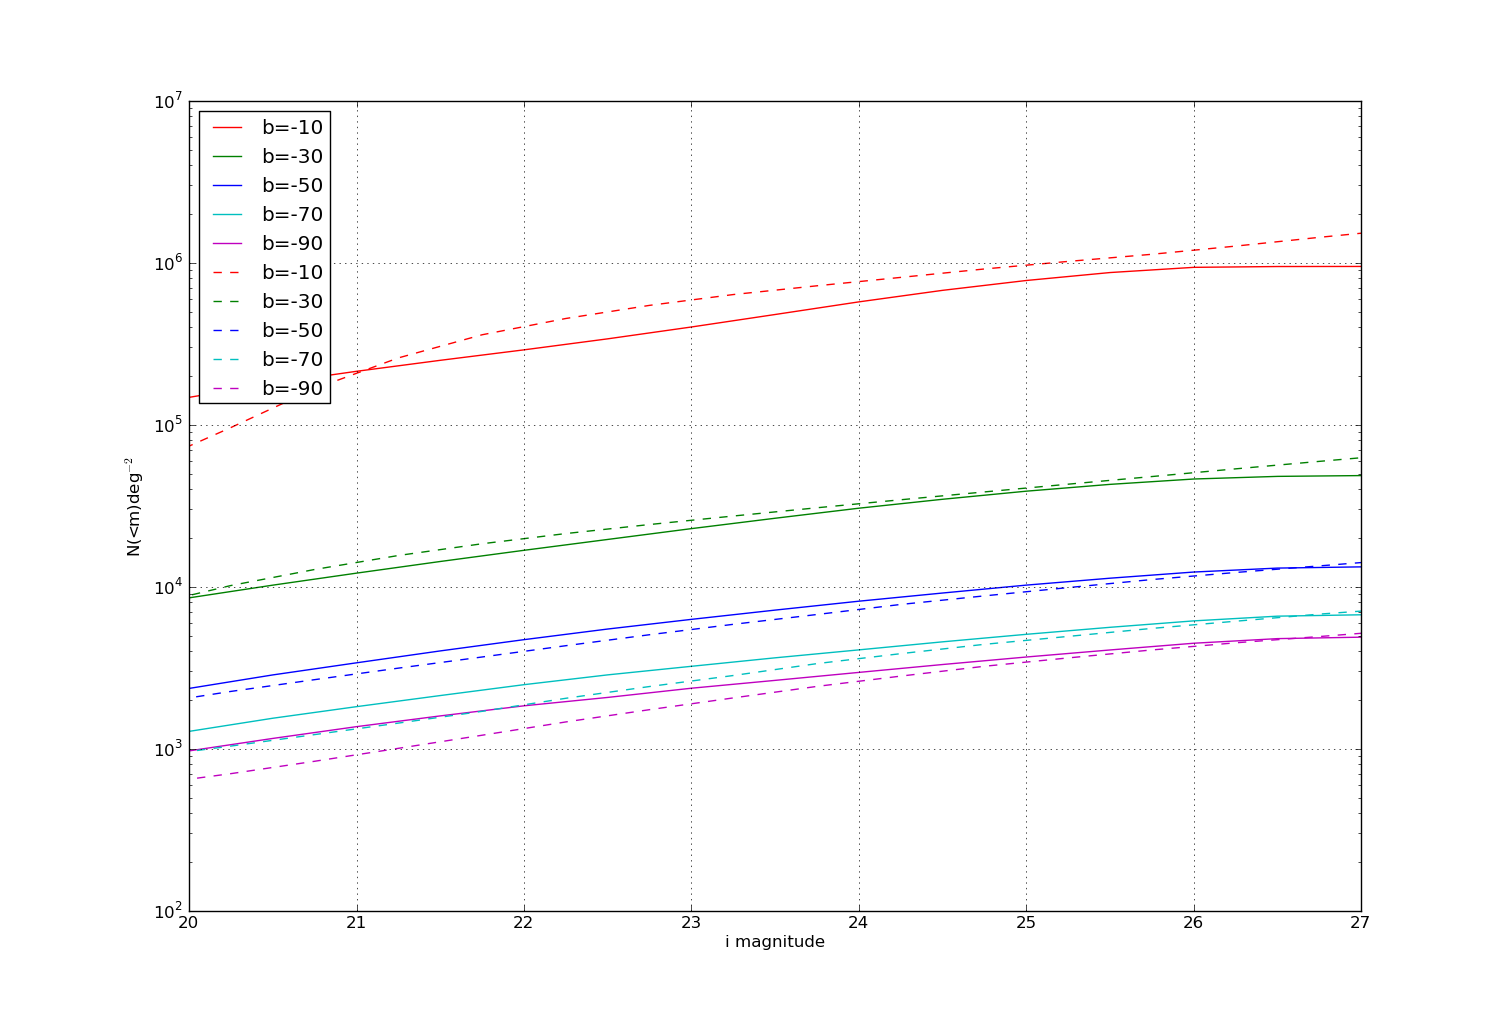
\includegraphics[width=5in]{validation_figures/cumulative_stars.eps}
\caption{Cumulative counts of stars from the Besancon (dashed) and Galfast (solid) models for 5 representative fields toward the galactic bulge \label{fig:scounts_0}}
\end{figure}
\begin{figure}
\centering
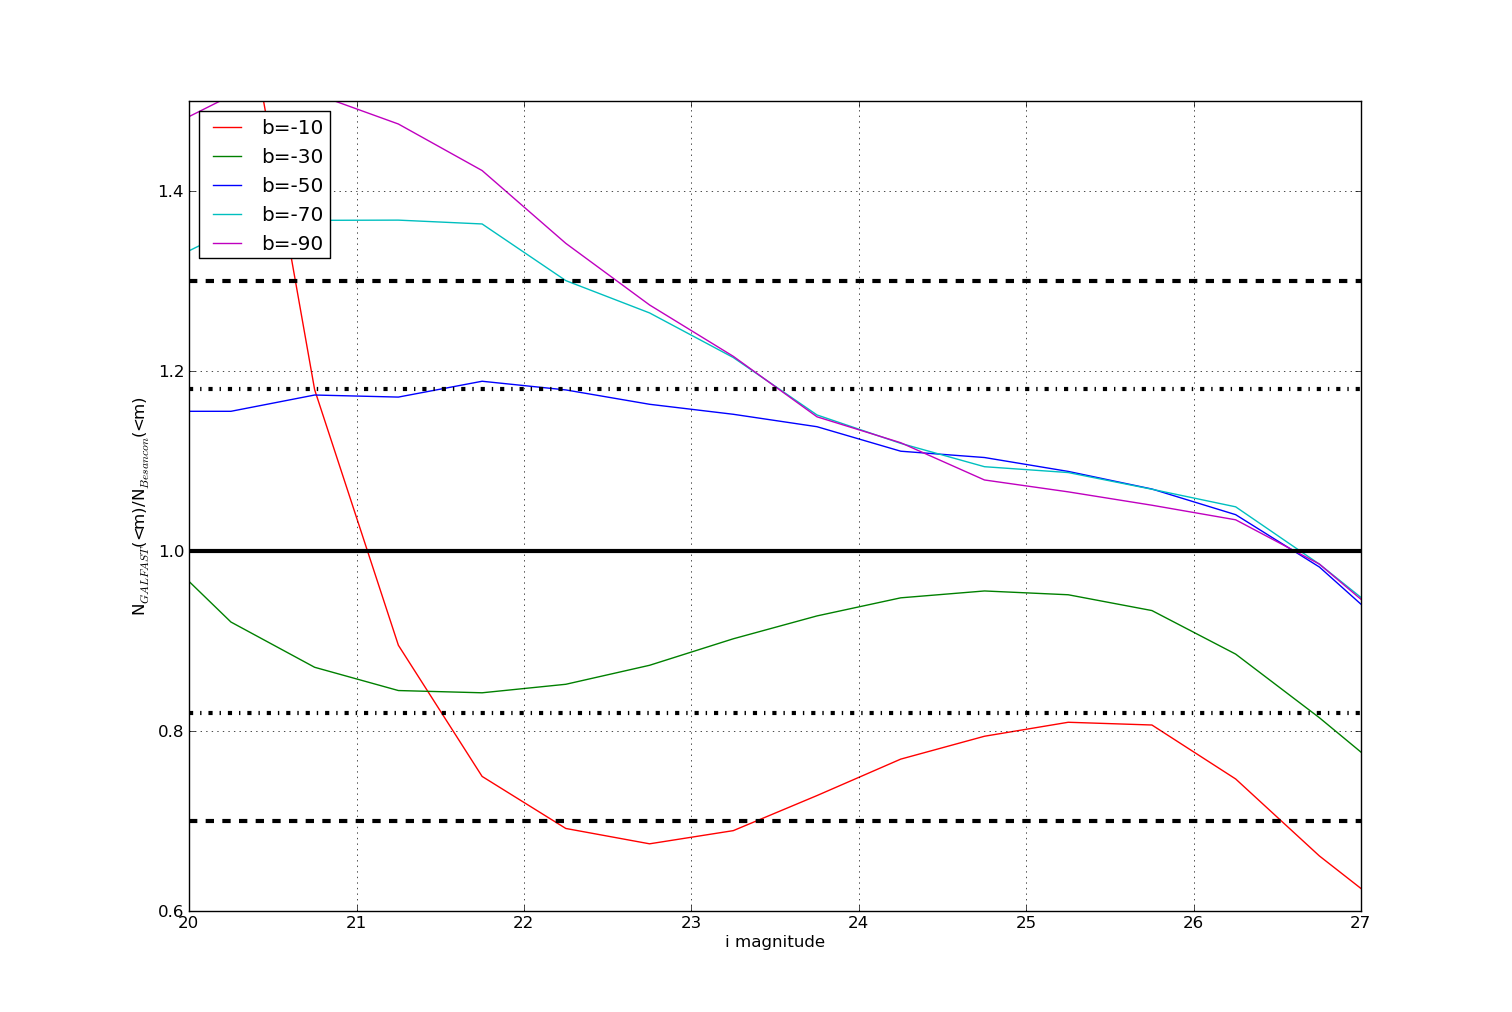
\includegraphics[width=5in]{validation_figures/cumulative_ratio_stars.eps}
\caption{Cumulative ratio of counts of stars from the Besancon and Galfast models for 5 representative fields toward the galactic bulge \label{fig:sratio_0}}
\end{figure}

\subsubsection{Galaxies \label{sec:galcounts}}
We compare the galaxy counts to those provided by the Durham group.  We have taken their compilations from:
{\tt http://star-www.dur.ac.uk/~nm/pubhtml/counts/idata.txt} access on 06/01/2013.  We use only data points with error bars in our analysis.  Using these counts
we noticed that the numbers of galaxies were under predicting at faint magnitudes.  We used a cloning algorithm to push up the number counts at faint magnitudes
while maintianing realistic number counts as a function of redshift.

The result of the nubmer counts as a function of magnitude after the cloning are shown in \ref{fig:gcounts}.  We have chosen the I-band data for comparison to 
minimize the effects of dust extinction which are somewhat uncertain in the Durham compilations.  A single transform of I$_{kc}$ = i$_{AB}$ - 0.5 was applied to
all compliation data.  For comparison with requirements on the sizing model stated in the requirements document, we also plot the cumulative ratio of the best fit polynomial
to the Durham data to the counts from the base catalog.  The goal is $\pm30\%$ to the coadded i-band depth of 26.8.  We see that the base catalog
underpredicts at the faintest magnitudes, but meets the requirement (Figure \ref{fig:gratio}).

\begin{figure}
\centering
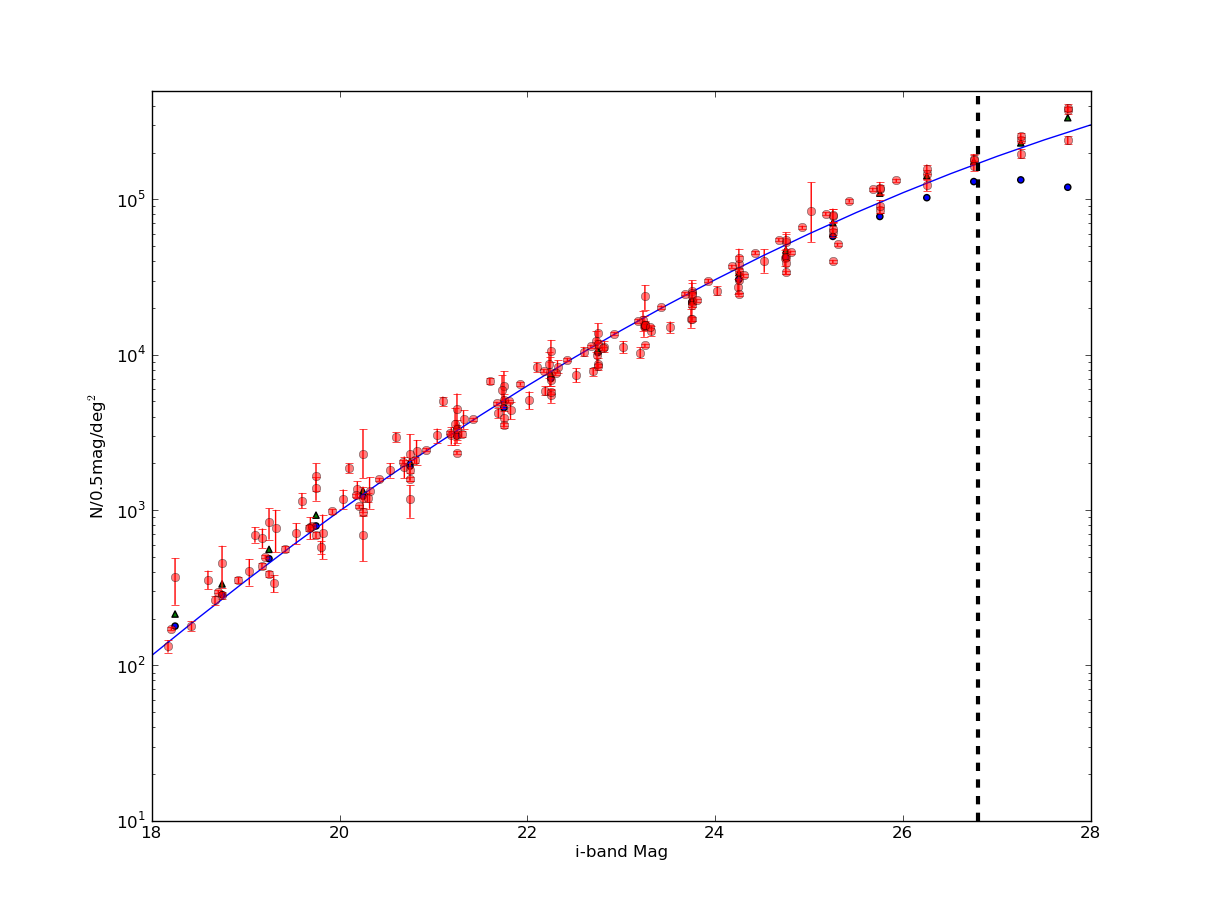
\includegraphics[width=5in]{validation_figures/Ngals-i.eps}
\caption{Durham counts (symbols) compared to the counts from the base catalog \label{fig:gcounts}}
\end{figure}
\begin{figure}
\centering
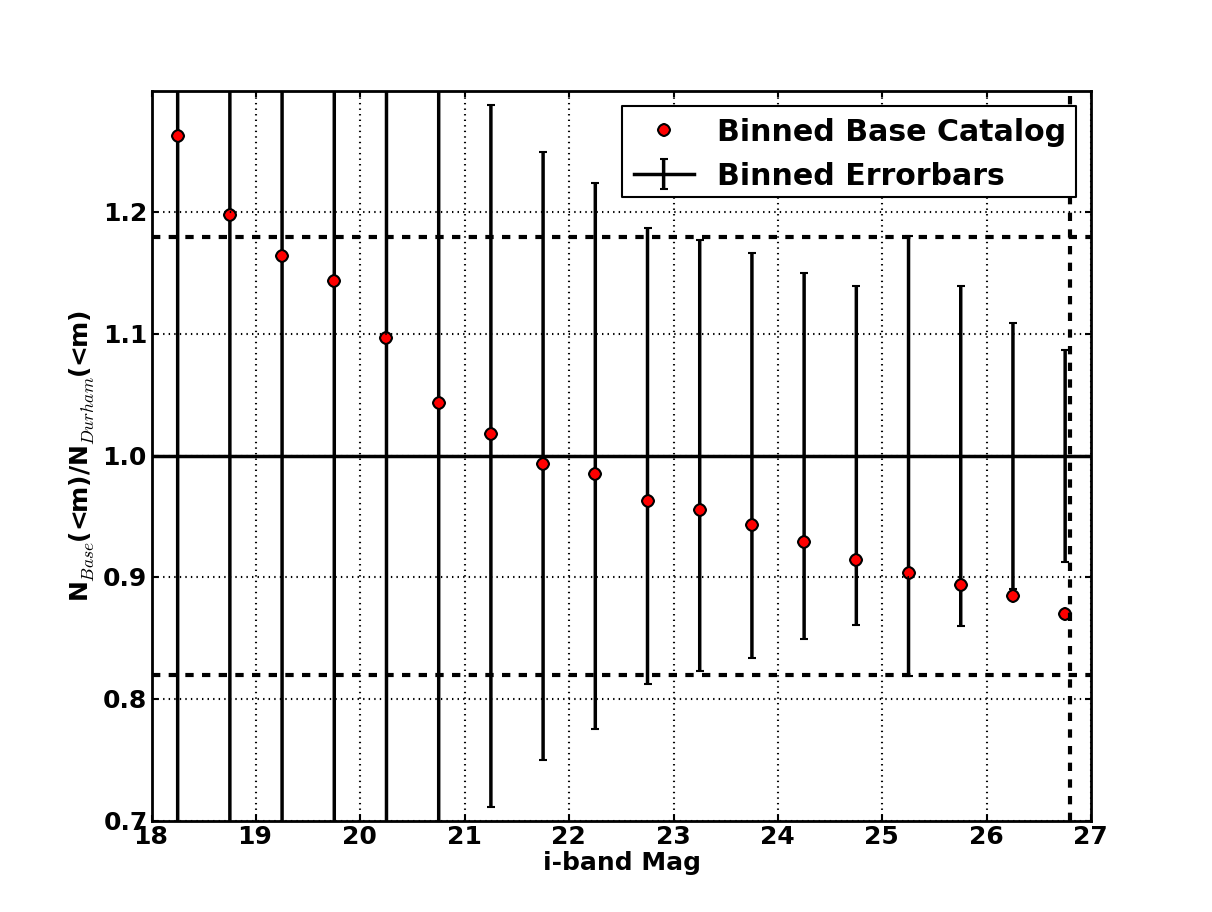
\includegraphics[width=5in]{validation_figures/CumulativeFraction_i.eps}
\caption{Durham counts divided by the counts from the base catalog.  Error bars are from adding the error bars from the data points in quadrature. \label{fig:gratio}}
\end{figure}

\subsection{Requirement 3: Size, ellipticity and redshift distributions of galaxies shall be representative of those observed by extant
telescopes and, for a fiducial image quality of 0.7 arcsec, deviations from the observed distributions shall
contribute $< 20\%$ of the observed effective density of galaxies, $n_{eff}$, used in the weak lensing samples (with a fiducial value of
$n_{eff} = 34$ galaxies per arcmin$^2$}
\subsubsection{Motivation}
One of the main science drivers for the LSST is the ability to conduct accurate weak lensing analysis.  Thus, the base catalogs must 
have fidelity better than the measurement errors and must represent a distribution of galaxies similar to observed distributions
so that measurement techniques can be compared directly to existing state of the art.  The measurement of weak lensing is dependent 
on the effective density of galaxies on the sky ($n_{eff}$).  The value of $n_{eff}$ depends on the inherent shape noise, the signal to noise distribution and the size distribution relative to the PSF.

The shape noise distributions was well measured by the COSMOS project and to first order is just the variance in the measured 
ellipticity distribution.  The $n_{eff}$ depends strongly on the apparent magnitude because of the steepness of the galaxy number
counts, but because of the dependence on signal to noise it has
has a very sharp cutoff at around i=24.5 {\bf Check this relative to Chihway's measure}.  Galaxy redshift distributions must
agree with observations to this limiting magnitude to assure accurate signal to noise distributions.  Finally, the size distribution
of the combined two component galaxy model must match measured distributions closely in order to reproduce predicted
values of $n_{eff}$ from measured distributions.  We measure the distribution from the base catalogs and show that it is well
within the envelope necessary to reproduce realistic values of $n_{eff}$.

\subsubsection{Measuring $n_{eff}$}
We use the framework described in \cite{chang} to calculate $n_{eff}$ for the distributions in the 
base galaxy catalog.  In summary, we use Equation 9 to calculate $n_{err}$:
\begin{equation}
n_{eff} = \frac{1}{\Omega}\sum^N_i\frac{\sigma^2_{SN}}{\sigma^2_{SN}+\sigma^2_{m,i}}
\end{equation}
where $\sigma_{SN}$ is the intrinsic shape noise and $\sigma_{m,i}$ is the shape measurement noise for the i$^{th}$ galaxy.

The shape noise is just taken from the ellipticity distribution.  For the distribution used in \cite{chang} $\sigma_{SN} = 0.26$.
The measurement noise can be approximated using Equation 13:
\begin{equation}
\sigma_m(\nu,R) = \frac{a}{\nu}\left[1+\left(\frac{b}{R}\right)^c\right]
\end{equation}
Where $\nu$ is the signal to noise ratio of the measurement, $R=\frac{r_{gal}^2}{r_{PSF}^2}$ is the relative size of the galaxy to
the point spread function.  We adopt the values from \cite{chang} of (a,b,c) = (1.58,5.03,0.39).  We choose a fiducial
PSF size of 0.7 arcsec. We use an estimate for the limiting magnitude of the coadded images on which the measurements are being
done of 26.7.  This takes into account the fact that the measurements are on extended sources as well as the fact that the SRD value 
of 27.5 in r is for dark sky observations at zenith.  We get this value by adjusting the limiting magnitude until our calculation
matches the value presented in \cite{chang} of 28. for the case of $k=1$.

For each galaxy $r_{gal}$ can be calculate from the flux ratio of the bulge and disk components as well as the effective half light 
radii of each component (see Appendix B in \cite{chang} for a derivation of this calculation).

Using this framework, we can test the sensitivity of the measured $n_{eff}$ on the ellipticity and size distributions.  For all calculations that follow we 
use the k=1 criterion meaning that galaxies with $\sigma_m < \sigma_{SN}$ are culled from the sample.

\subsubsection{Galaxy radius measurements}
There are many definitions of galaxy size: half light radius, first moment radius, second moment radius, Petrosian radius, Kron radius, etc.
We must choose one of these measurement to compare to observed data.  One aspect informing which measurement we use is whether it is included 
in our reference catalog.  We have chosen to use the COSMOS ACS catalog \cite{cosmos} because of the size ($~2deg^2$), depth ($~26.$ in i), and
quality (space based).  

The COSMOS catalog reports the second moments and the 
half light radius, so either the second moment radius or half light radius could be used for comparison.  A major concern is that the measurements
on the base catalog are effectively infinite signal to noise, whereas the measurements from COSMOS are not.  We find that the second moment 
radii are strongly affected by noisy measurements where the half light radius is much less sensitive.  To test this, we sample from truncated Sersic
profiles for each galaxy.  The truncation determines where the profile falls below the noise as the noise should contribute to the moments symmetrically.
As the truncation shrinks we see that both the width and mean of the second moment radius distribution decrease.  We see this in the
half light radius distribution as well, but at a much lower level.  See Figure \ref{fig:mom_hist} and Figure \ref{fig:hl_hist}.  Figure
\ref{fig:mom_hl_line} shows that the half light distribution shape measurements are flat down to truncation at 3 half light radii, where 
the second moment radius distribution is not stable even going from 100 to 10 half light radii.  For these reasons, we choose to compare the half light 
radius distribution to the half light radius distribution from the COSMOS catalog.
\begin{figure}
\centering
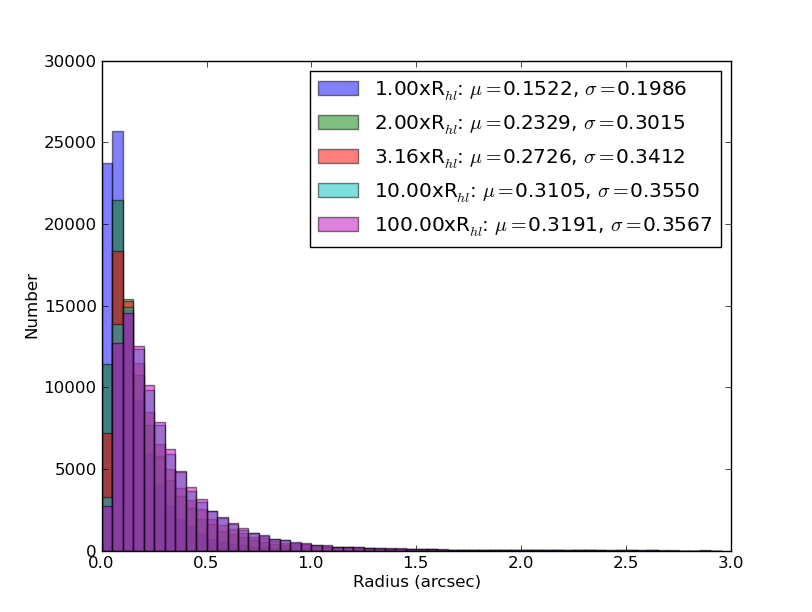
\includegraphics[width=5in]{validation_figures/half_light_hist.eps}
\caption{\label{fig:hl_hist}}
\end{figure}
\begin{figure}
\centering
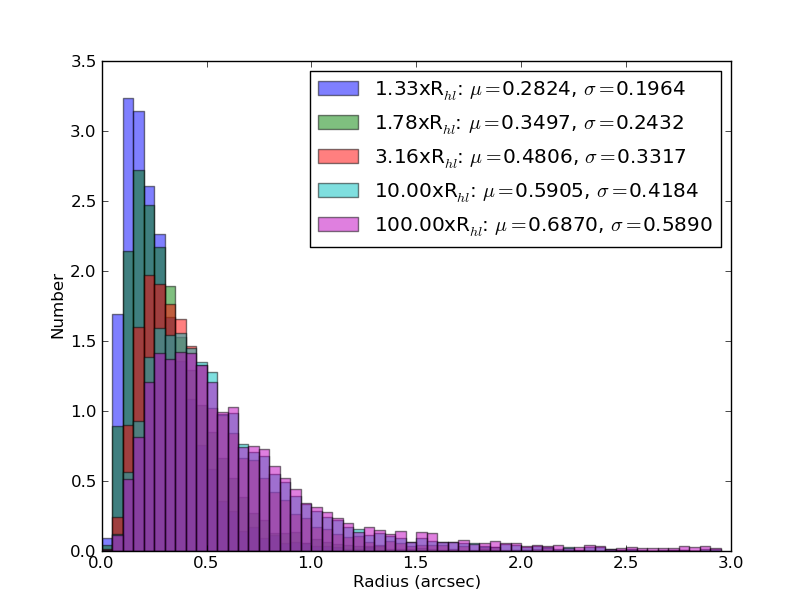
\includegraphics[width=5in]{validation_figures/Second_moment_hist.eps}
\caption{\label{fig:mom_hist}}
\end{figure}
\begin{figure}
\centering
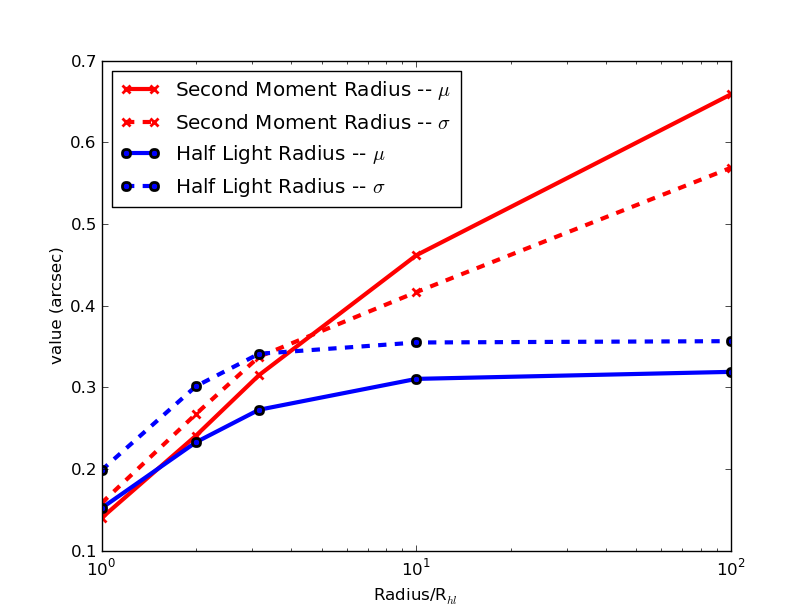
\includegraphics[width=5in]{validation_figures/sec_mom_half_light_mean_sigma.eps}
\caption{\label{fig:mom_hl_line}}
\end{figure}

To test the sensitivity of $n_eff$ on the input half light radius distribution, we model the the half light distribution as a log normal distribution (see Figure
\ref{fig:hl_dist}).  Assuming that half light distribution is driven by the disk components, we choose the bulge distribution from the base catalog and then
choose a lognormal distribution with varying shape parameters to probe the size distribution space.
\begin{figure}
\centering
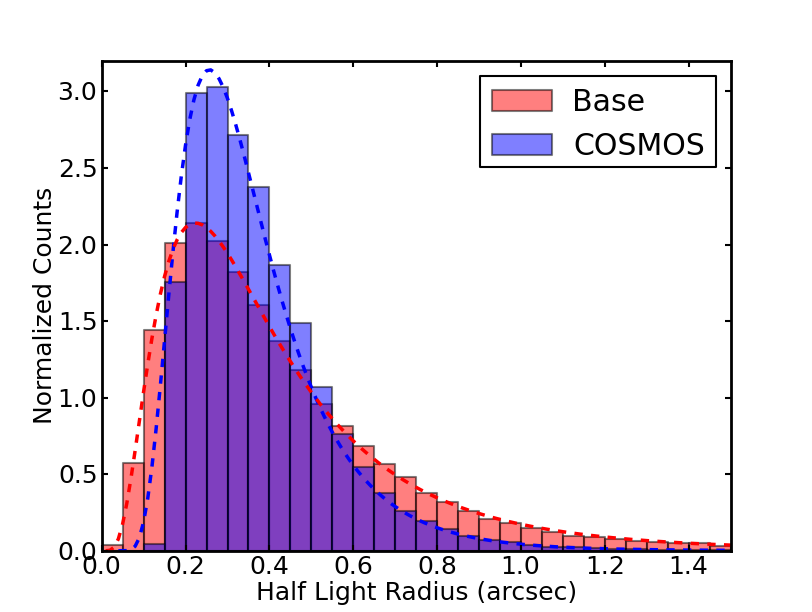
\includegraphics[width=5in]{validation_figures/ln_fit.eps}
\caption{{\bf XXX This figure needs to be remade, it was done with only objects 20 - 24.5.}\label{fig:hl_dist}}
\end{figure}

Figure \ref{fig:size_sens} shows the sensitivity to the size distribution.  The x axis is related to the width of the 
distribution and the y axis is related to the location of the peak of the distribution. Over-plotted are points corresponding
to the best fit log normal distributions to the COSMOS data set, the base catalog data set, and the base catalog data set convolved 
with a 0.1 arcsec psf.
\begin{figure}
\centering
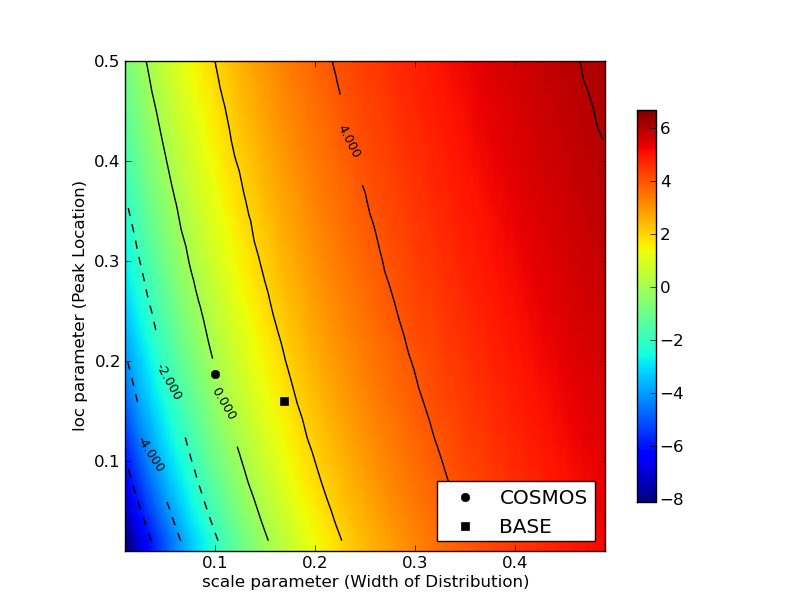
\includegraphics[width=5in]{validation_figures/size_sensitivity.eps}
\caption{{\bf XXX This figure needs to be remade, it was done with only objects 20 - 24.5.}\label{fig:size_sens}}
\end{figure}

\subsubsection{Measurement of shape noise.}
Our ellipticity distribution is far narrower than that measured by the COSMOS survey.  This has direct impact on the measured
$n_{eff}$ through the intrinsic shape noise term.  I'm in the process of trying to correct for this, and will flesh this out when that is done.


%\begin{figure}
%\centering
%\includegraphics[width=5in]{validation_figures/COSMO_base_ellip.eps}
%\caption{\label{fig:ellip}}
%\end{figure}
\subsubsection{Redshift distributions}
The redshift distributions are in very good agreement with the \cite{coil} empirical redshift distributions.
\begin{figure}
\centering
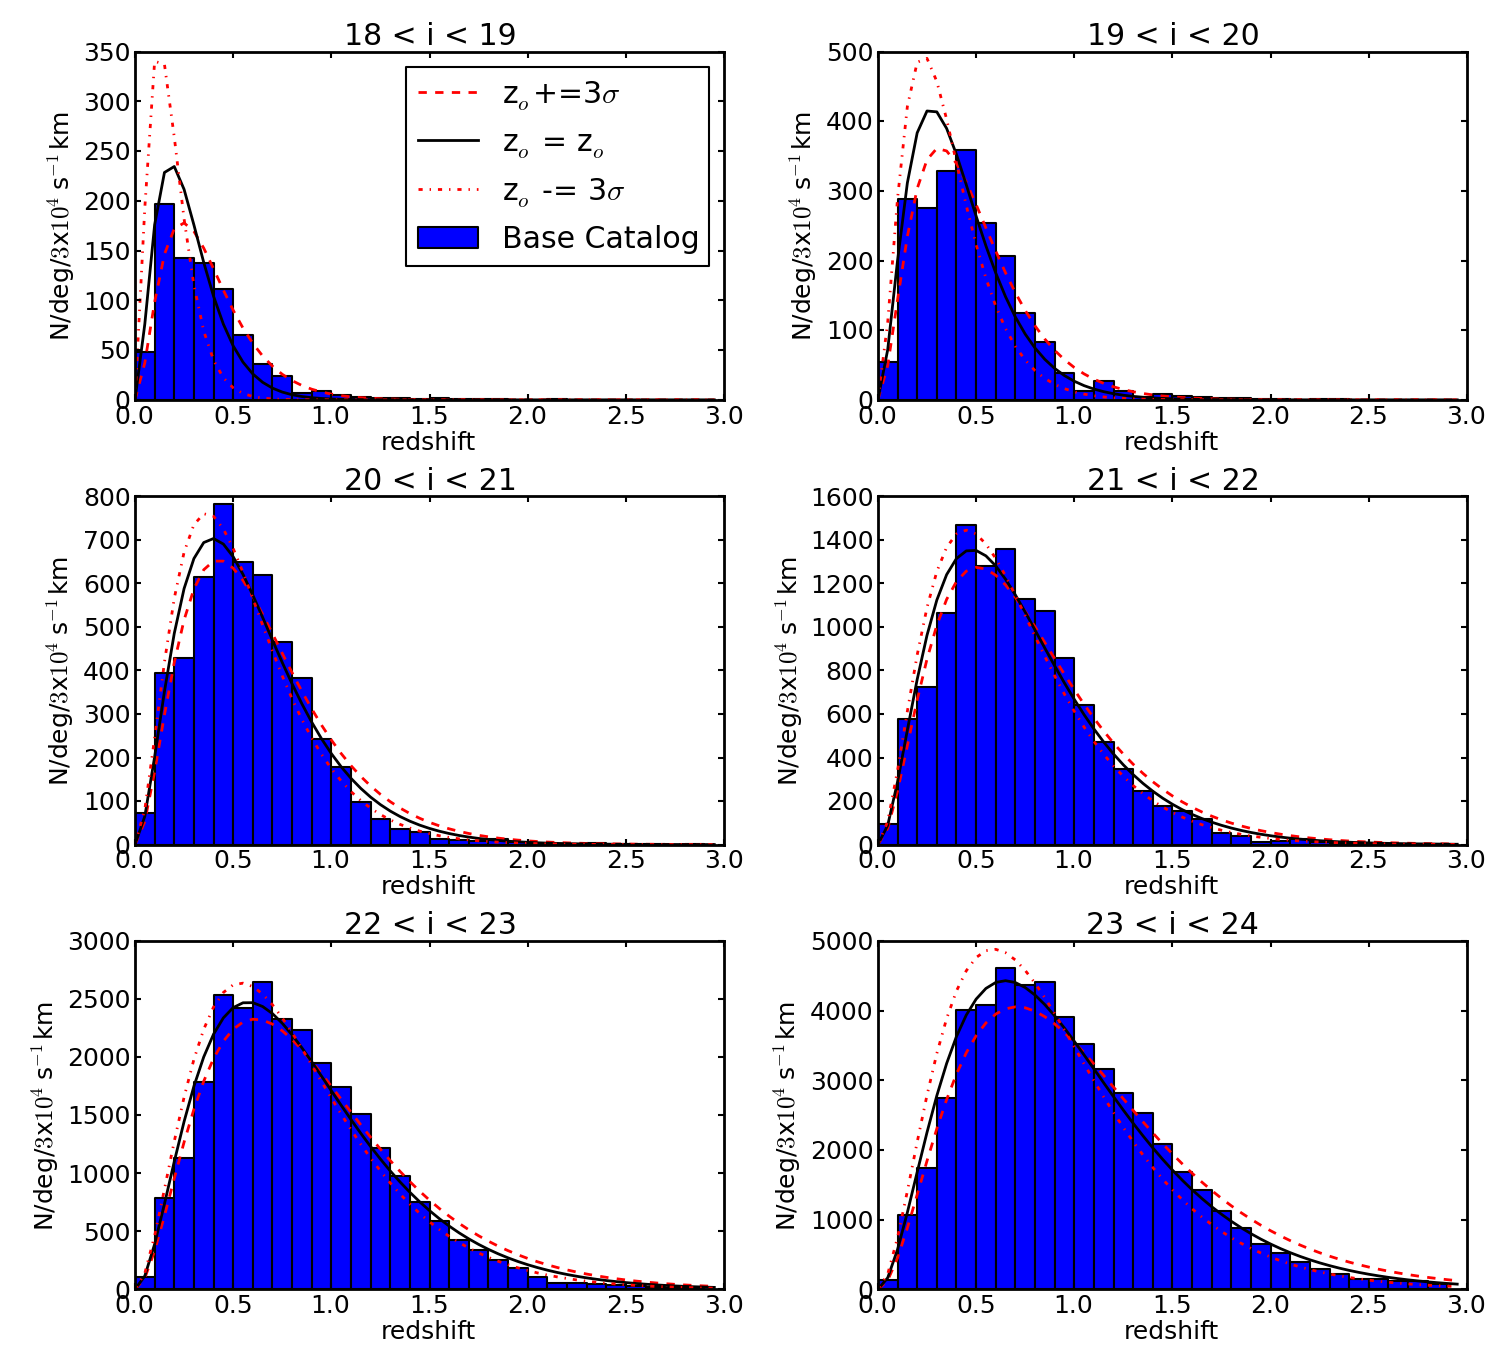
\includegraphics[width=5in]{validation_figures/Nofz_18_24.eps}
\caption{N(z) for 18 to 24 with distribution from \cite{coil}\label{fig:nofz18_24}}
\end{figure}
\begin{figure}
\centering
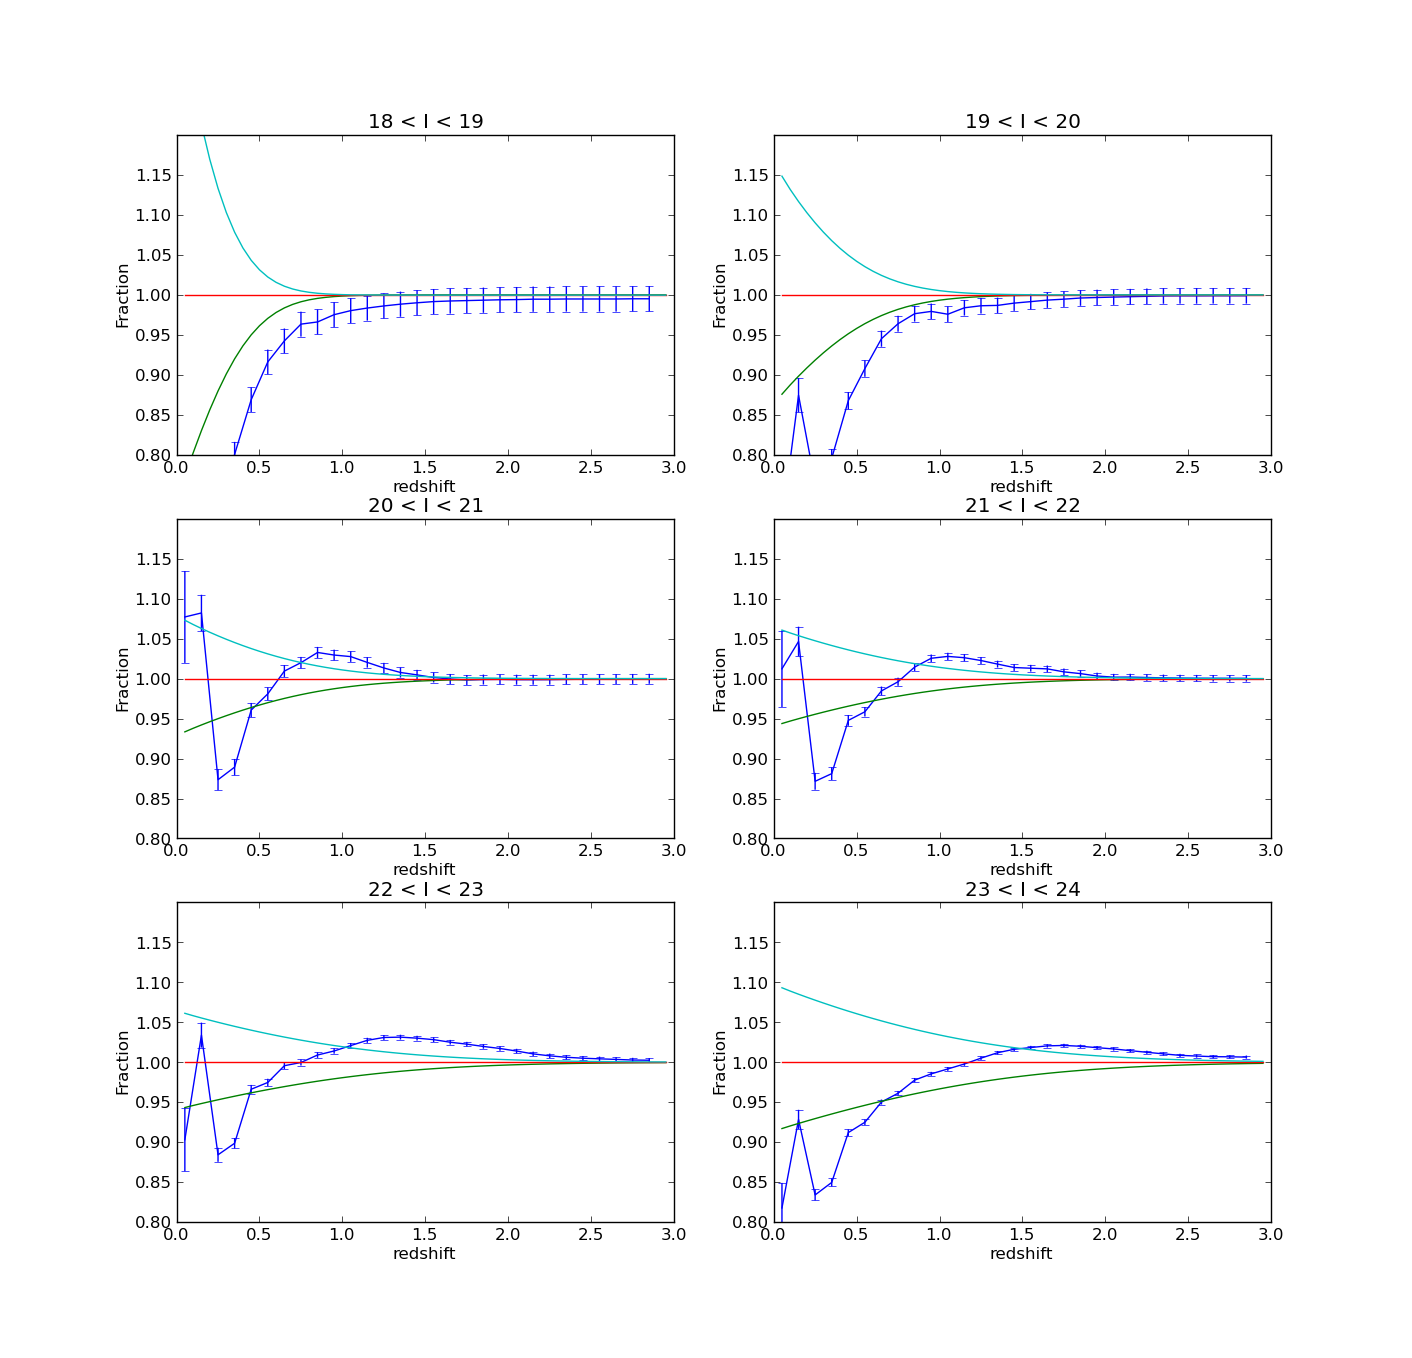
\includegraphics[width=5in]{validation_figures/Nofz_CumulativeFraction_18_24.eps}
\caption{N(z) for 18 to 24 with distribution from \cite{coil}\label{fig:nofz18_24_ratio}}
\end{figure}
\begin{figure}
\centering
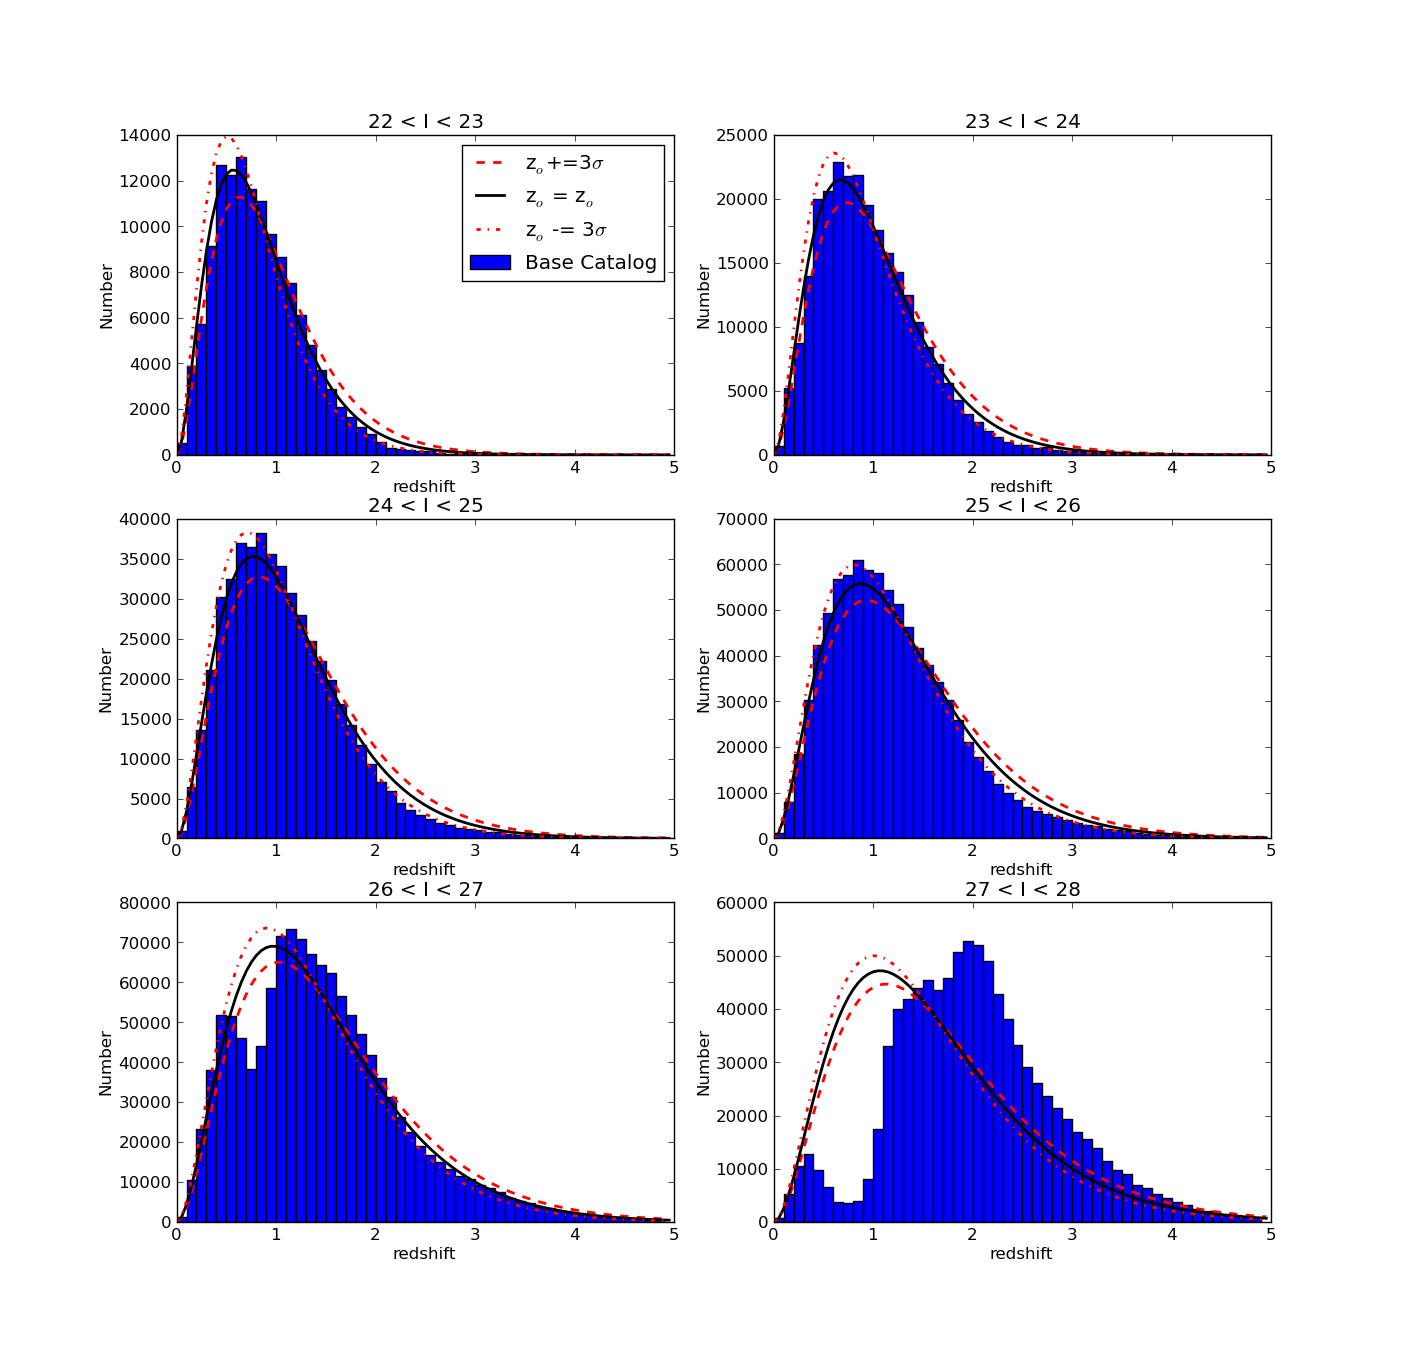
\includegraphics[width=5in]{validation_figures/Nofz_coil_22_28.eps}
\caption{N(z) for 22 to 28 with distribution from \cite{coil}\label{fig:nofz22_28}}
\end{figure}
\begin{figure}
\centering
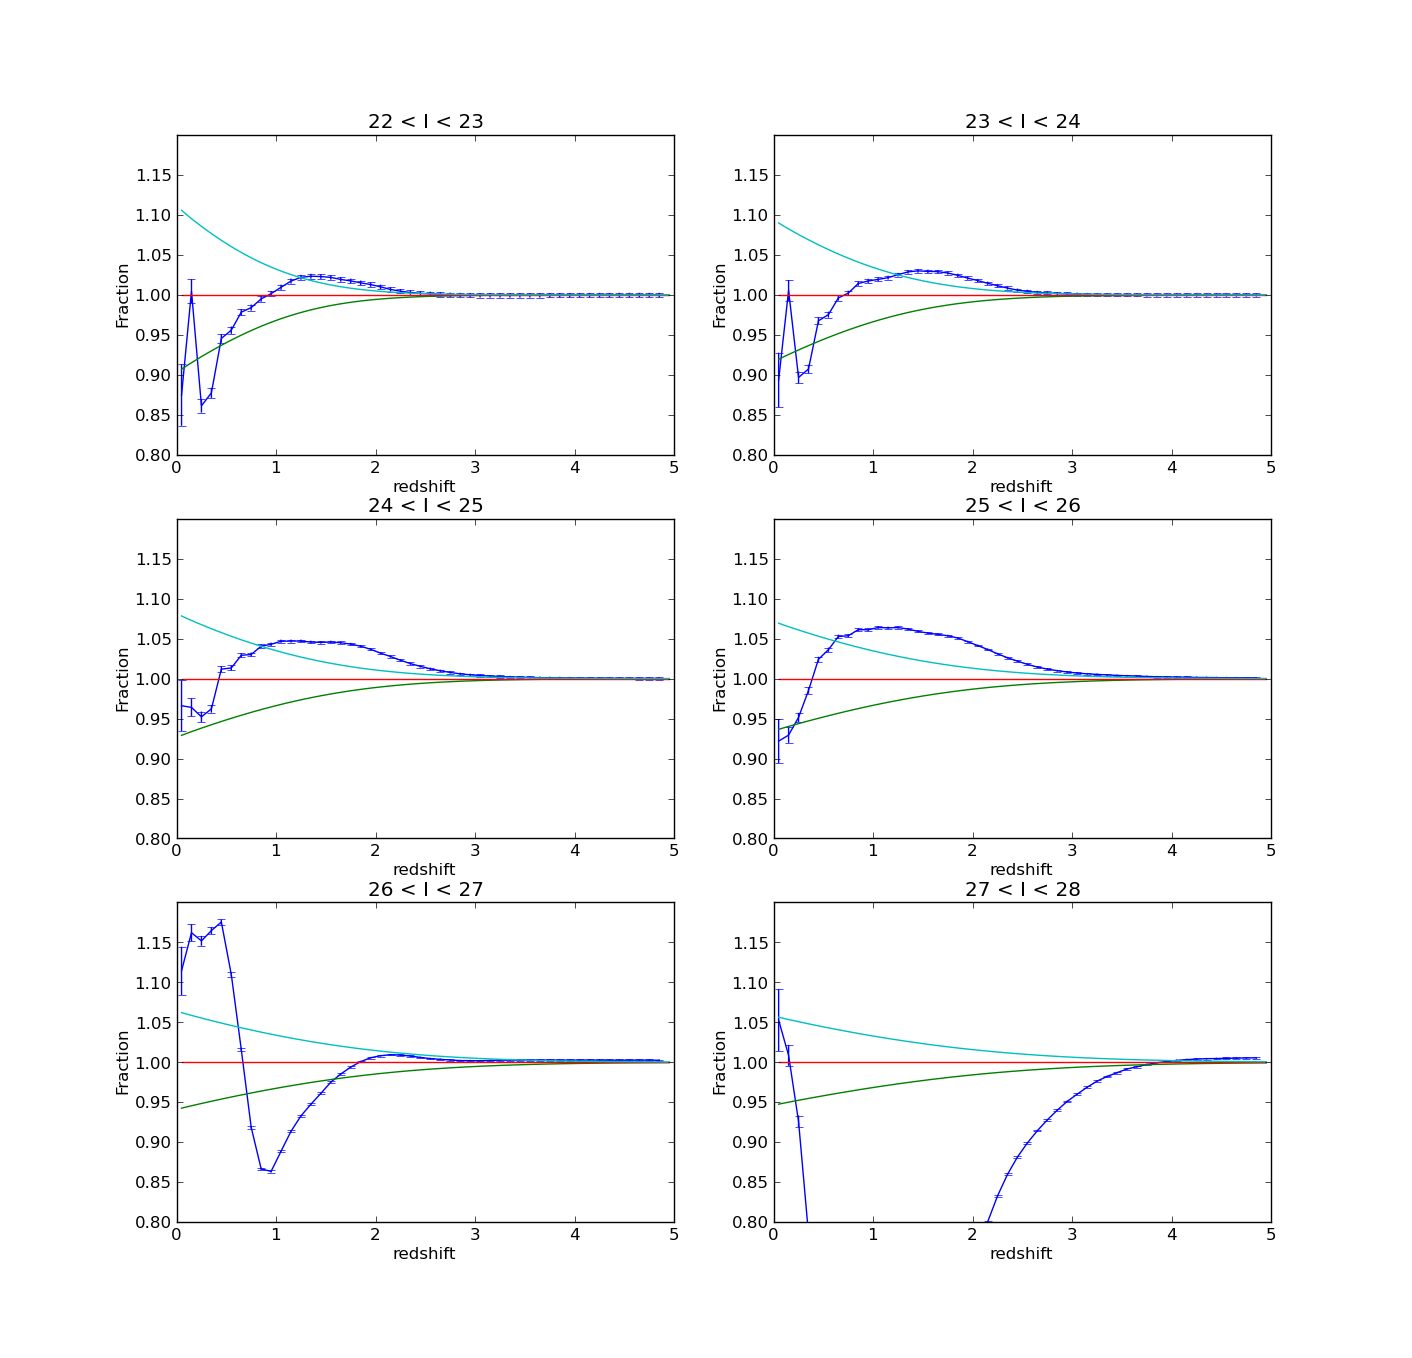
\includegraphics[width=5in]{validation_figures/Nofz_CumulativeFraction_22_28.eps}
\caption{N(z) for 22 to 28 with distribution from \cite{coil}\label{fig:nofz22_28_ratio}}
\end{figure}

\subsection{Requirement 4: For the photometric calibration simulations
the distribution of stellar colors shall encompass the colors of white dwarfs through red giant branch stars.
The median color distributions of stars must trace the observed color locus for these stars to within 0.02 magnitudes
of the principal color (s,w,x,y) to the designed 5$\sigma$ single epoch limiting magnitude in the r-band.
{\bf update this for the most recent statement in the requirements document}}
For several reasons from calibration through to stellar populations work the Galactic model must have realistic color distributions.
This goes beyond simply spanning the proper color ranges.  The main sequence stellar locus must also agree with the location of the
stellar locus from other projects.  In Figure \ref{fig:starcolorspan} we show that the more trivial requirement that the stellar
colors span the ranges given in the requirements document is met.  Dashed lines in each panel show the requirements.  The measured
color distribution is plotted in the histogram.  The main sequence and red giant branch (RGB) contributions are plotted separately from
the white dwarf population.  Together the two distributions cover the required range.  The y-axis is log scale.

To verify the veracity of the main sequence stellar locus, we use the principal colors of the stellar locus defined by \cite{ivezic04}.
We use stars selected from the same fields as used in the number counts analysis for all fields south of a galactic latitude of -30.
In order to avoid complications associated with the difference between the LSST and SDSS photometric systems, we calculate the un-extincted 
magnitudes in the SDSS bandpasses using the best fit spectrum for each star.  We then calculate
the principal colors for each star using the relations in \cite{ivezic04}, but removing the r-band dependence in $P\prime_{2}$.  Figure
\ref{fig:principalcolors} shows that the principal colors as calculated from the base catalog are in very good agreement with
the location of the stellar locus in the SDSS (zero color).  The base catalog easily meets the requirement of $\pm0.02mag$ deviation
from the stellar locus to single epoch depth in all 4 principal colors.  The scatter and trend with magnitude in the s color is due to 
the sensitivity of u-band on $[$Fe$/$H$]$.  Figure \ref{fig:sfeh} shows this dependence.  The transition from high metalicity disk stars to low 
metalicity halo stars introduces the scatter and slope.

Figure \ref{fig:principalcolorshist} shows that the requirement of mean deviation from the color locus defined by the four principal colors by less than 
0.02 magnitudes is met in all four bands.
\begin{figure}
\centering
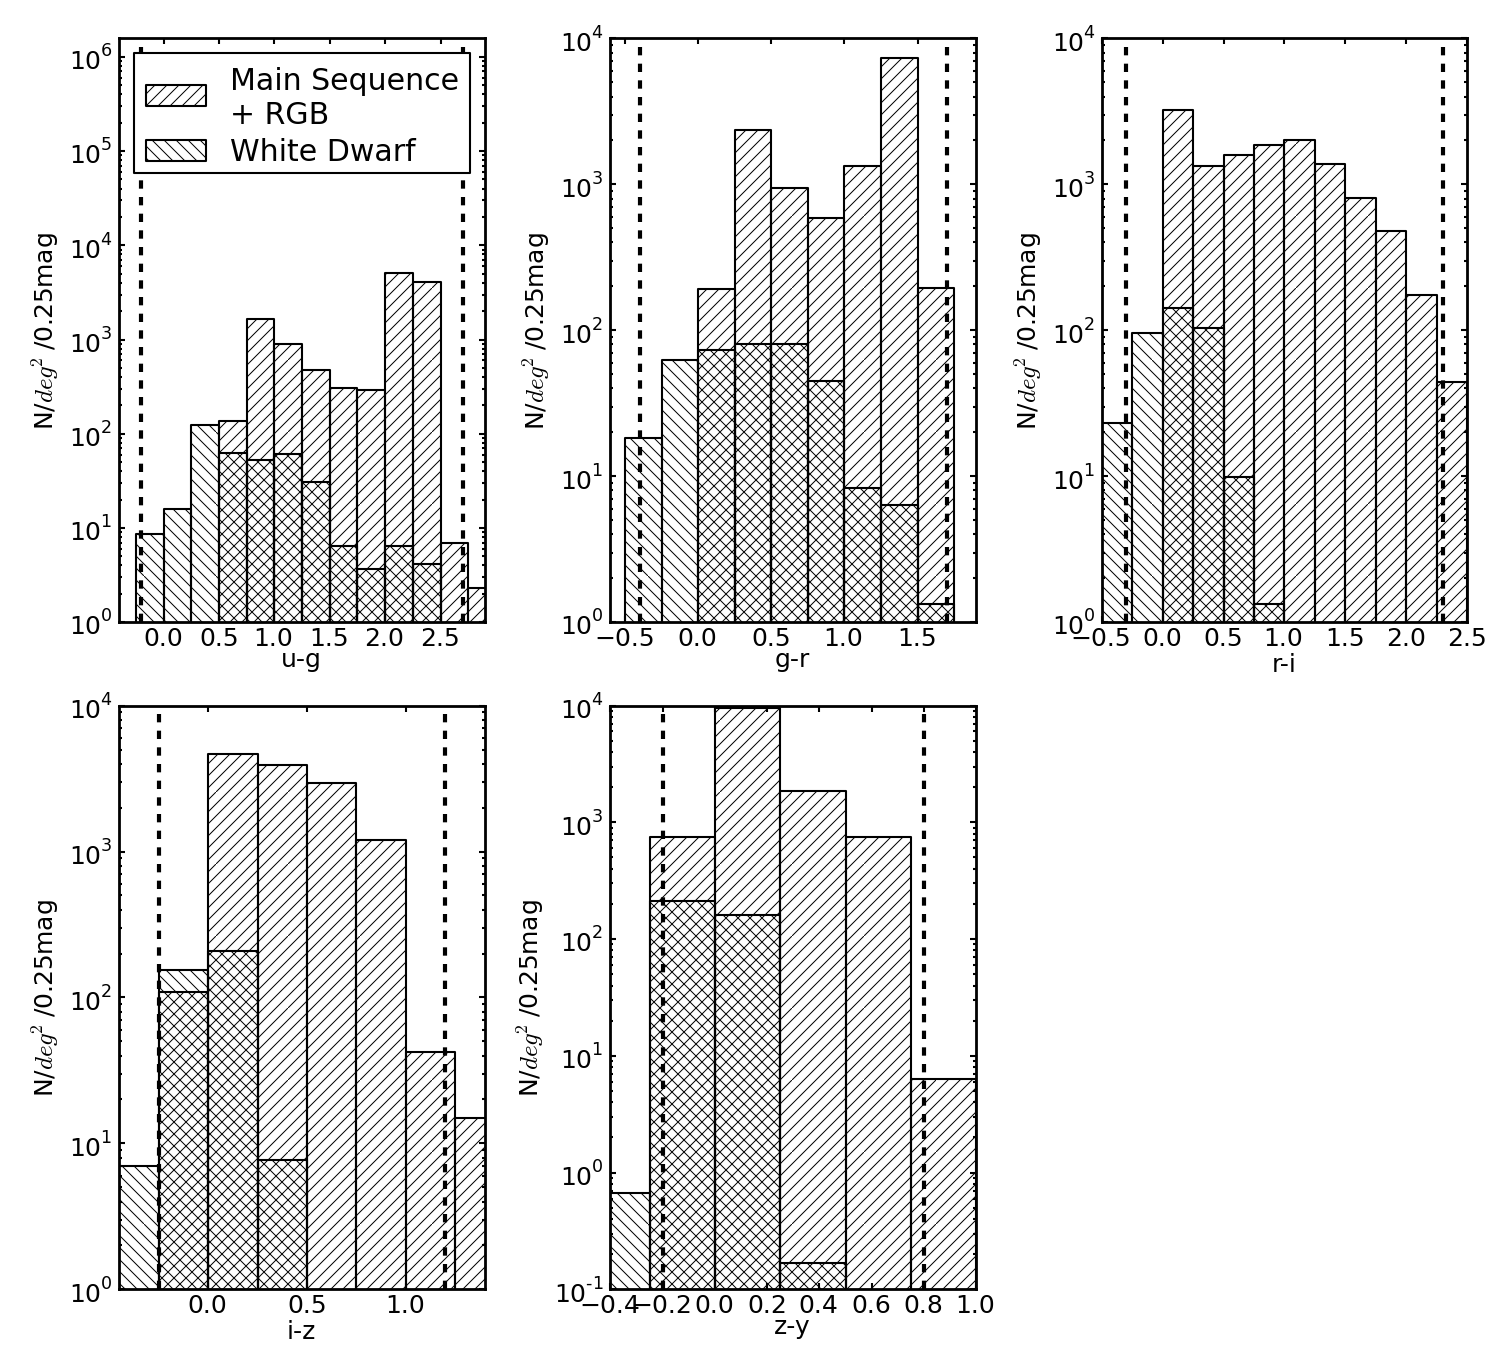
\includegraphics[width=5in]{validation_figures/star_lsst_color_hist.eps}
\caption{{\bf XXX make sure these are actually normalized} Normalized counts of main sequence, red giant branch and white dwarf stars.  Heavy dashed lines show the requirements stated in the requirements document.\label{fig:starcolorspan}}
\end{figure}

\begin{figure}
\centering
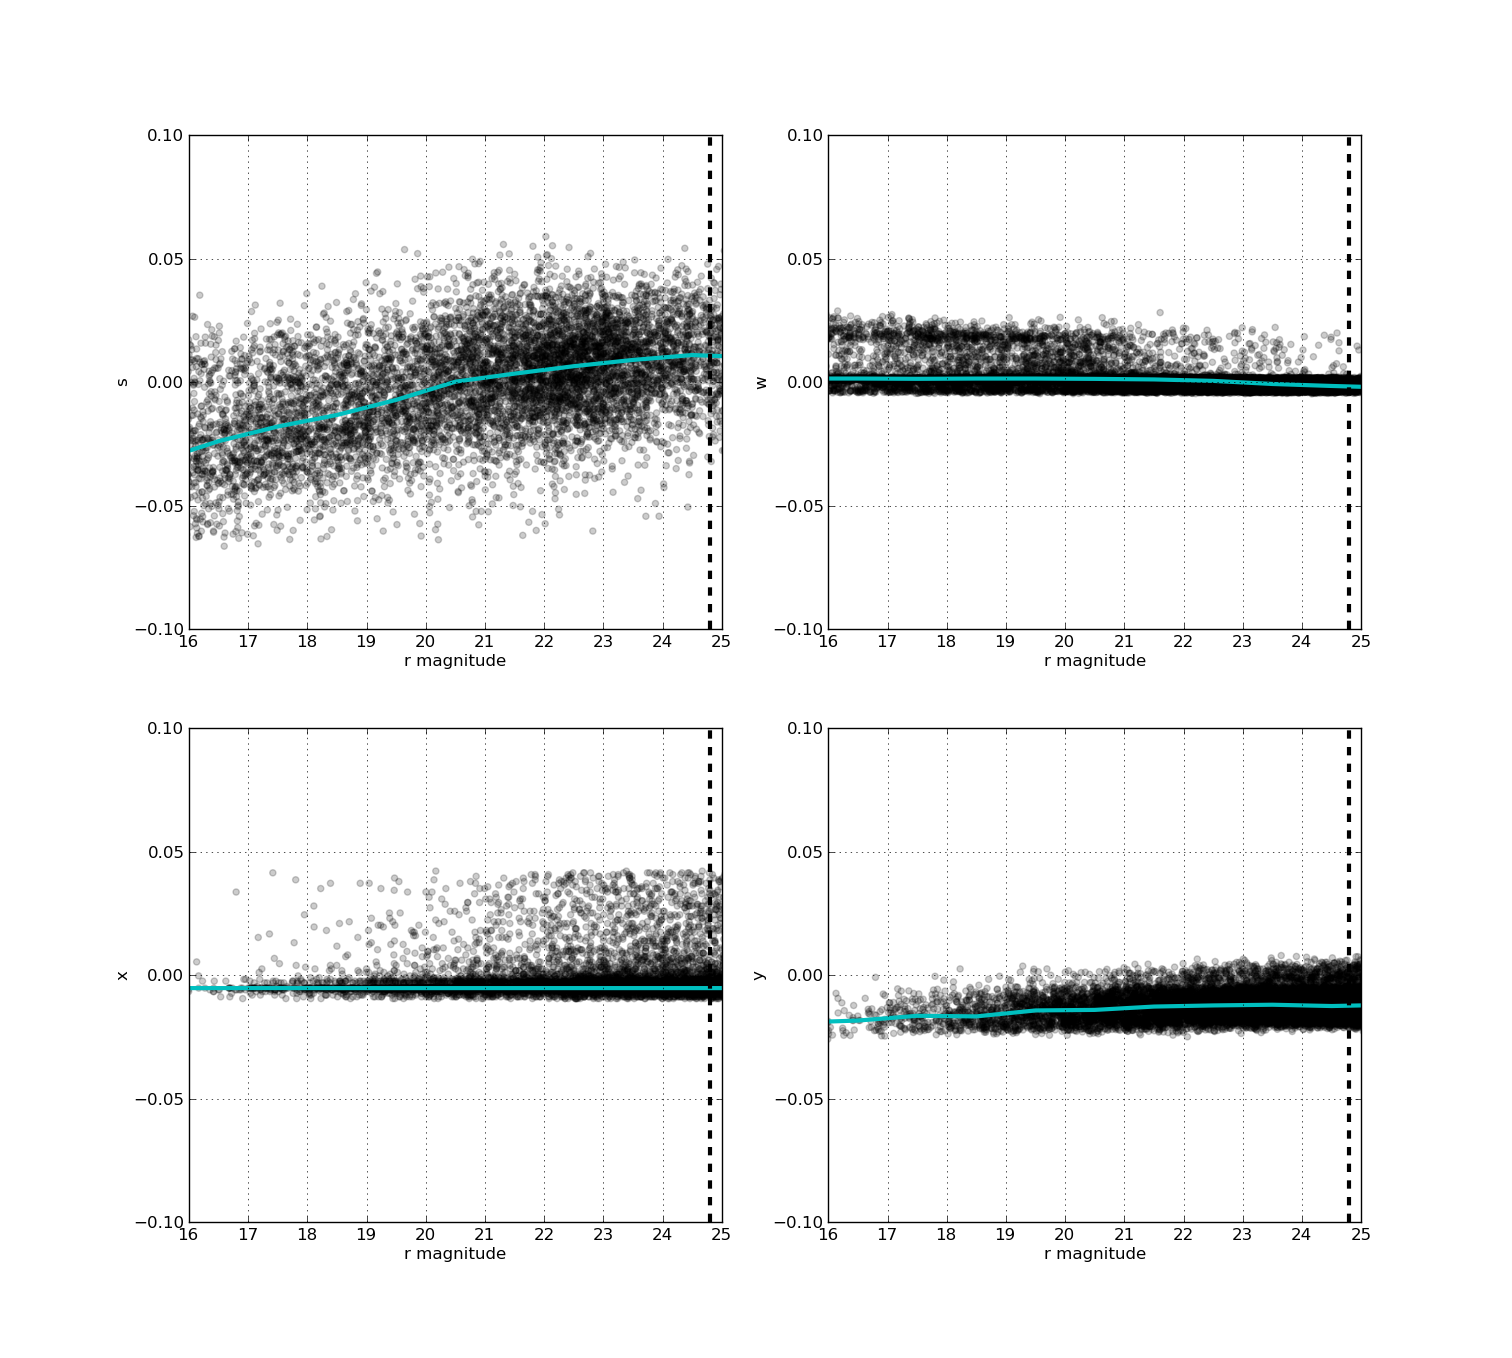
\includegraphics[width=5in]{validation_figures/principal_colors_vr.eps}
\caption{Principal colors for the base catalog compared to the location of the stellar locus in the SDSS.\label{fig:principalcolors}}
\end{figure}

\begin{figure}
\centering
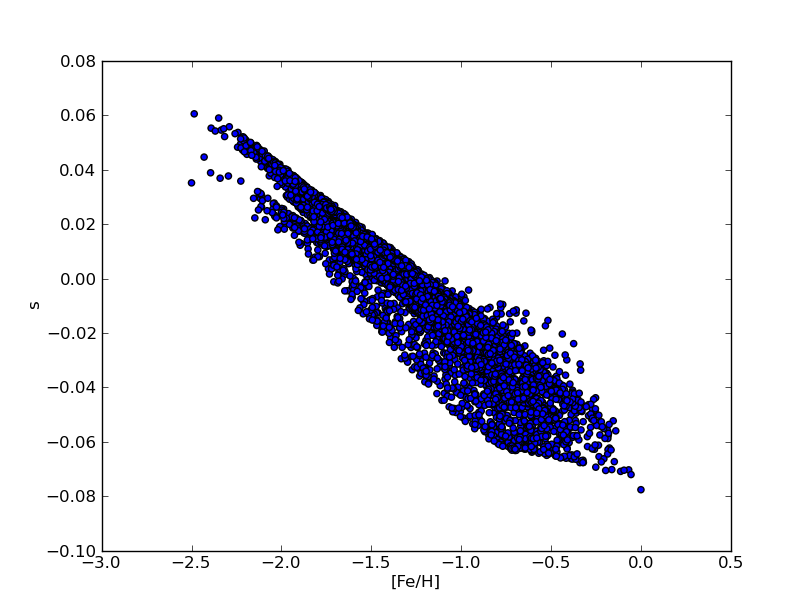
\includegraphics[width=5in]{validation_figures/s_met.eps}
\caption{The principal color 's' as a function of metalicity.\label{fig:sfeh}}
\end{figure}

\begin{figure}
\centering
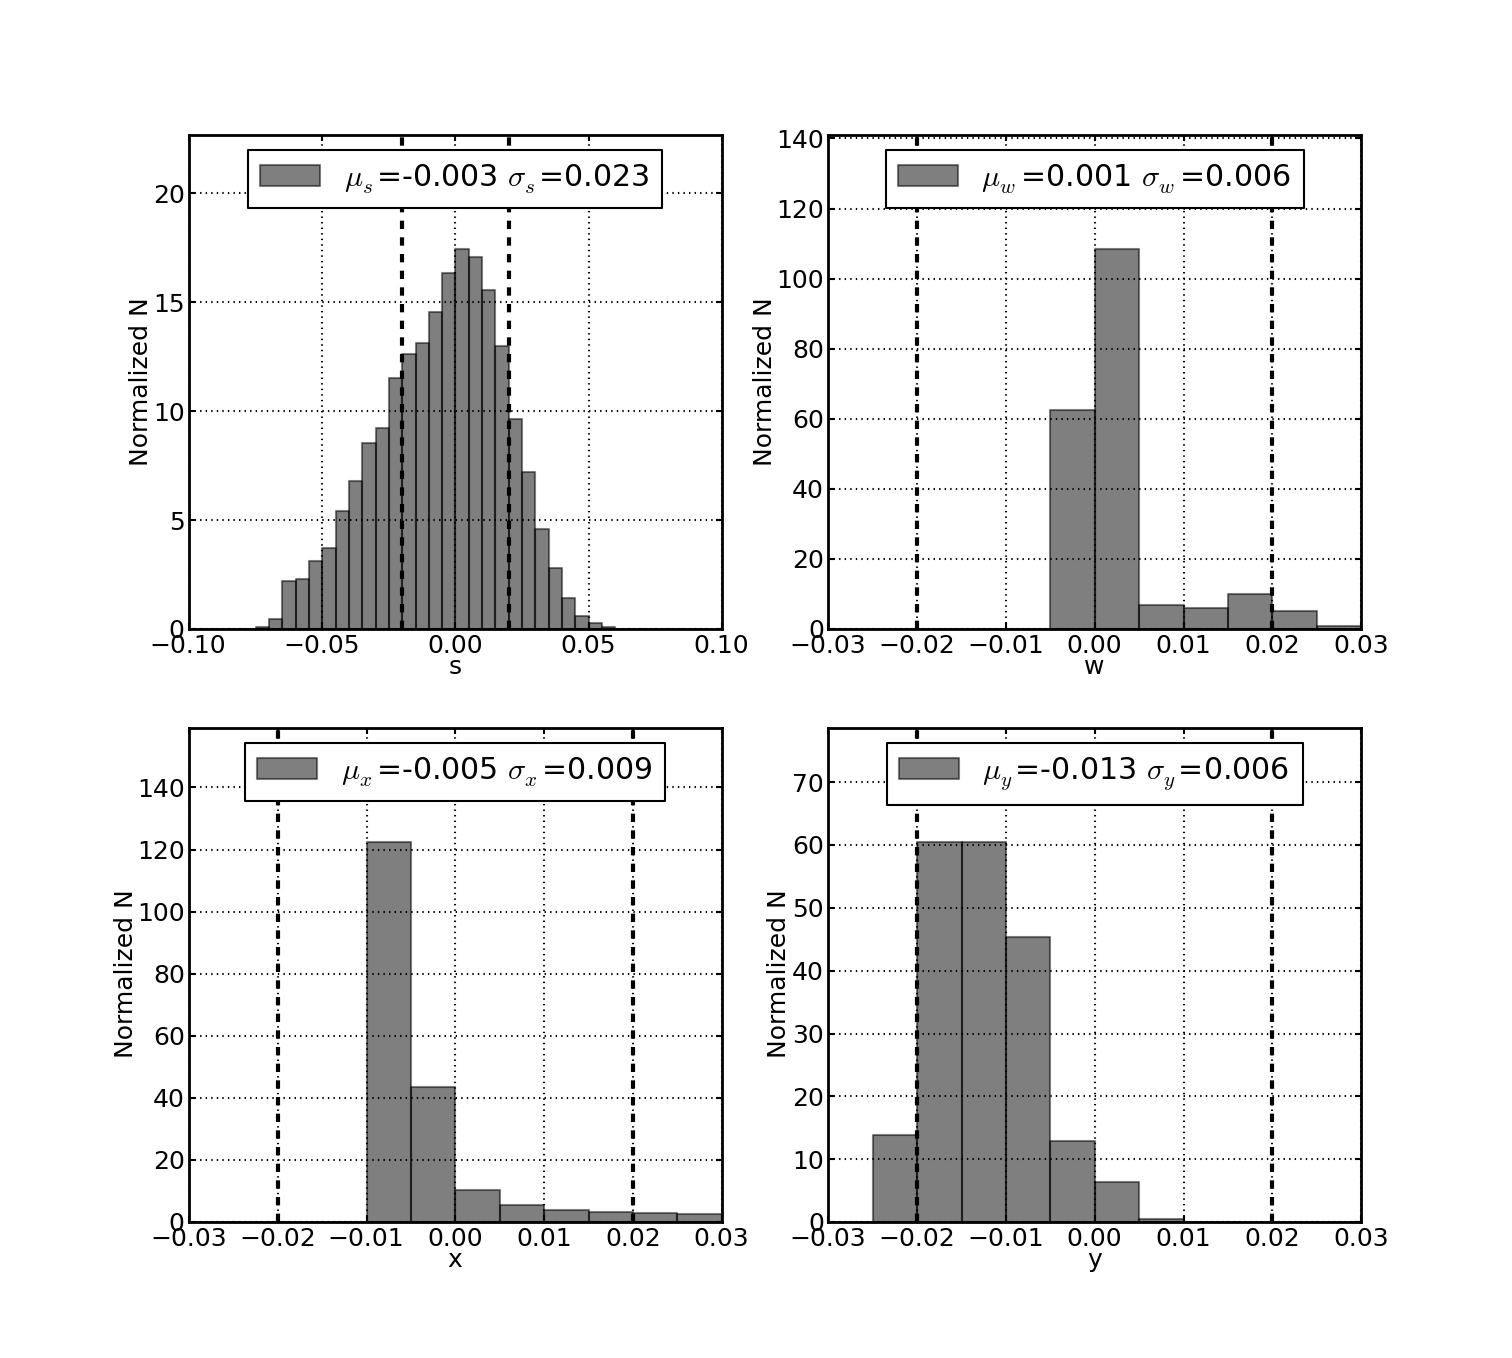
\includegraphics[width=5in]{validation_figures/principal_colors_hist.eps}
\caption{Hisograms of the principal colors of stars in the base catalog to the stretch depth of r < 24.8. The mean and standard deviation for each 
histogram are given in the legend in the upper right.\label{fig:principalcolorshist}}
\end{figure}
\subsection{Requirement 5: All models for the astrometric transforms applied tothe catalogs (including interpolation functions) 
shall have an accuracy better than 1.6 mas}
{\bf XXX Need help from AJC and Yusra on this one.}
\subsection{Requirement 6: The system shall be capable of incorporating new astrophysical catalogs without requiring
a redesign of the class-schema framework}
The ability to create new catalogs is available within the framework by the creation of user-designed subclasses and class mixins. A new type of catalog can be generated as a new class using the InstanceCatalog base class and other user-designed catalog classes (also using the InstanceCatalog base class) and class mixins. The columns desired in the new catalog are defined as class attributes. The data for these columns is gathered from the database directly or using methods defined in the class
for the catalog itself, in class mixins designed by the user, or in the base classes. These data gathering methods can take the form of a "get\_'column\_name'" method or in the form of compound columns with their own "get\_" methods. The required database column is then referred to in the "column\_by\_name()" method which returns the column values from the database. For example, the CustomCatalog below uses various aspects of this framework to write a new catalog to file:

\begin{verbatim}
class BasicCatalog(InstanceCatalog):
    """Simple catalog with columns directly from the database"""
    catalog_type = 'basic_catalog'
    refIdCol = 'id'
    column_outputs = ['id', 'ra_J2000', 'dec_J2000']
    # transformations specify conversions when moving from the database
    # to the catalog.  In this case, we take RA/DEC in radians and convert
    # to degrees.
    transformations = {"ra_J2000":np.degrees,
                       "dec_J2000":np.degrees}

class AstrometryMixin(object):
    @compound('ra_corrected', 'dec_corrected')
    def get_points_corrected(self):
        ra_J2000 = self.column_by_name('ra_J2000')
        dec_J2000 = self.column_by_name('dec_J2000')
    # ... do the conversions: these are just standins
    ra_corrected = ra_J2000 + 0.001
    dec_corrected = dec_J2000 - 0.001
    return ra_corrected, dec_corrected

class CustomCatalog(BasicCatalog, AstrometryMixin):
    catalog_type = 'custom_catalog'
    refIdCol = 'id'
    column_outputs = ['id', 'redshift', 'points_corrected']
    transformations = {"ra_corrected":np.degrees,
                       "dec_corrected":np.degrees}

# Now to create a catalog, we connect to a database and call write_catalog
db = GalaxyObj()
catalog = CustomCatalog(db)
catalog.write_catalog("out.txt")

# out.txt has the following columns:
# id redshift ra_corrected dec_corrected
\end{verbatim}

The InstanceCatalog metaclass verifies that all new columns desired in the user-defined catalog have associated means of gathering the required data from the database. If no method exists nor is there an associated database entry for the column directly then an error is raised. Furthermore, the error is raised before data begins transfer from the database because the instantiation of the class initiates a dry run of the table output. After the dry run the necessary database columns are verified
against the actual columns in the database and if there is a discrepancy the error is raised. As a result, the user is protected from errors after the data is pulled from the database and since all the necessary columns are determined during the dry run only one single query of the database is required to pull all necessary data.
\end{document}
